%!TEX root = ../thesis.tex
%*******************************************************************************
%****************************** Third Chapter **********************************
%*******************************************************************************
\chapter{Planificación y estado de avance.}

% **************************** Define Graphics Path **************************
\ifpdf
    \graphicspath{{Chapter5/Figs/Raster/}{Chapter5/Figs/PDF/}{Chapter5/Figs/}}
\else
    \graphicspath{{Chapter5/Figs/Vector/}{Chapter5/Figs/}}
\fi

Es posible pensar en este proyecto de Tesis, como un conjunto de postulaciones y planteamientos de nuevas metodologías basadas en el uso de técnicas de minería de datos que permitan estudiar mutaciones en conjuntos de datos y que culminan con una gran temática, que aborda la implementación de una herramienta computacional para el diseño de mutaciones.

Dado esto, el proyecto en sí, puede dividirse en tres grandes objetivos, de los cuales, los conocimientos y destrezas adquiridas en los primeros dos, son necesarias para cumplir con el tercer gran objetivo. Esto, es posible observarlo en la Figura \ref{cap5:fig1}.

\begin{figure}[!h]
	
	\centering
	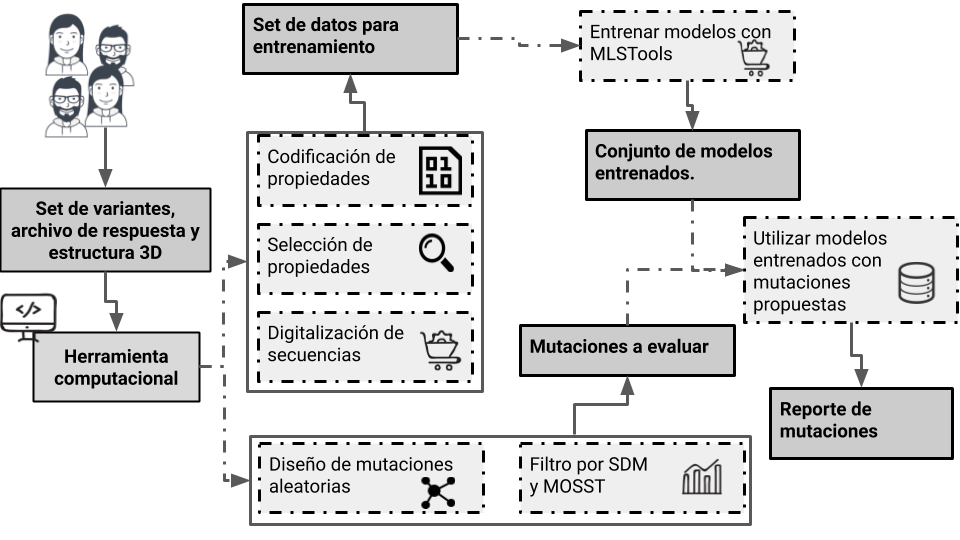
\includegraphics[scale=.5]{fig1.png}
	\caption{Esquema representativo de objetivos generales involucrados en el desarrollo del proyecto.}
	\label{cap5:fig1}
\end{figure}

El primer objetivo, se basa en la construcción de modelos de clasificación o regresión basados en algoritmos de aprendizaje supervisado, enfocados en el estudio de mutaciones puntuales en una proteína y cómo afectan éstas en términos de una respuesta conocida. Esto va en directo beneficio del estudio de nuevas mutantes o variantes en proteínas de interés, apoyados en una metodología que maximiza el desempeño de los modelos. 

Por otro lado, el segundo objetivo se basa principalmente en representar secuencias lineales de proteínas a partir de la digitalización de propiedades fisicoquímicas y empleando transformadas de Fourier como representación de espectros de frecuencias. Si bien, el enfoque principal es la representación en sí, el objetivo también abarca el cómo utilizar estas representaciones para el entrenamiento de modelos de clasificación o el reconocimiento de patrones e identificación de residuos que aportan a las propiedades fisicoquímicas.

